\documentclass[UTF8,fontset=fandol,11pt,a4paper]{ctexart}
\usepackage[margin=23mm]{geometry}
\usepackage{amsmath,amssymb,booktabs,graphicx,xcolor,hyperref,fancyhdr}
\definecolor{ink}{HTML}{23364A}
\definecolor{accent}{HTML}{167D9A}
\hypersetup{colorlinks=true,linkcolor=accent,urlcolor=accent,citecolor=accent,pdftitle={变散热边界下的热模型降阶与误差控制},pdfauthor={徐楷沅 2352163}}
\setlength{\parindent}{2em}
\setlength{\parskip}{0.35em}
\clubpenalty=10000
\widowpenalty=10000
\pagestyle{fancy}\fancyhf{}\fancyhead[L]{\small Moonshine 热仿真研究}\fancyhead[R]{\small 徐楷沅 · 2352163}\fancyfoot[C]{\thepage}
\setlength{\headheight}{15pt}
\title{\color{ink}变散热边界下的热模型降阶与误差控制\\[4mm]\large 基于 Moonshine 的可复现研究}
\author{徐楷沅\quad 学号：2352163}
\date{2026 年 10 月 25 日}
\begin{document}
\maketitle
\begin{center}\color{accent}\textbf{课程研究报告\quad 数学模型 · 真实迭代 · 冻结实验 · 独立复核}\end{center}
\begin{abstract}
本研究从课程 EDA 资料中的热仿真加速问题出发，在二维线性稳态导热模型上研究变化散热边界引起的降阶失效。原版 Moonshine 生成并执行求解器、POD 基线、失效分析及自适应内核，外部提供评测驱动与独立复核。冻结方法后，在三个网格、256 个参数组成的同一查询序列上各完成三次计时。固定 8 维 POD 分别有 6、6、7 例场误差超过 $10^{-3}$；带解析屏障触发和基增广的方法未观察到超标。计入必要离线成本后，自适应方法在 24 次查询时比快速完整求解更慢，在 256 次查询时的成本比中位数分别为 4.455、5.295、5.392。全部 15、15、17 次回退均为保守触发，说明误差指标仍有改进空间。结果限定于合成离散模型和本机实验，不代表连续温度认证或工业难题已完全解决。
\end{abstract}
\section{研究问题与范围}
本课题来源于课程资料《难题：EDA 专题第四期 2026.06.01》第 4 页的“热仿真加速”。原题涉及大规模网格、变化的换热系数、非线性材料及工业计算资源约束。本研究选取其中的一个有限数学子问题：在固定二维线性稳态导热模型中，散热边界变化会怎样影响固定降阶空间的准确度；能否用可计算的误差指标触发完整求解和基更新，并在计入全部成本后取得收益？

研究对象是无量纲合成模型，不包含真实芯片几何、流固耦合或工业实测数据。误差容限 $\tau=10^{-3}$ 表示无量纲温升误差，不能解释为 $1\,{}^{\circ}\mathrm{C}$。评价重点是明确假设、可复现实验、失败案例与智能体迭代，原工业题的完整解决不在已完成工作的声称范围内。

\section{Moonshine 的执行与成果归属}
研究使用 \href{https://github.com/DeepMathLLM/Moonshine}{DeepMathLLM/Moonshine} 原版研究流程，固定上游提交为
\href{https://github.com/DeepMathLLM/Moonshine/tree/bb0e4aa025fdcc5297fff1025ab4876f120ed615}{\texttt{bb0e4aa025fd}}（完整标识见运行证据），上游跟踪源码未修改。本地启动器负责选题、会话恢复、预算与证据快照；模型适配器通过本机已登录的 Codex CLI 提供文本、拟调用工具及结构化审核响应。工具执行仍由 Moonshine 的原版运行时承担。

每一研究单元按“读取题面与记忆、问题质量评估、生成程序、实际运行、检查与修订、局部审核、归档”推进。\texttt{assess\_problem\_quality} 评估问题是否值得研究，\texttt{run\_python\_script} 产生可核对的退出码及数值输出，\texttt{verify\_overall} 提供假设、计算和逻辑方面的模型审核。质量评估与模型审核均不等于形式化证明，阶段编号也不自动表示完成度。

成果按来源区分：求解器、POD 基线及失效分析程序由 Moonshine 生成和执行；题面、文献核查、解析屏障先验与测试协议审阅由外部协调和独立复核提供。Moonshine 对输入的屏障进行了推导核对、实现和有理数检查，因此该部分是有来源的协作研究，不是智能体自主发现的新通用定理。外部复核脚本单独存放，不计为 Moonshine 的原生执行次数。每轮保存输入、工具事件、代码快照、审核与归档记录；接口错误、未定审核和后续修订均保留。

\section{导热模型与守恒离散}
在 $\Omega=(0,1)^2$ 上求相对环境温升 $T$：
\begin{equation}
 -\nabla\!\cdot(k\nabla T)=q,\qquad
 -k\nabla T\cdot\boldsymbol n=h_sT\quad\text{于边界段 }s,
 \label{eq:thermal-pde}
\end{equation}
其中 $k=1$，四边参数按左、右、下、上排序，$\mu=(h_L,h_R,h_B,h_U)\in[0.2,5]^4$。源项在 $[0.2,0.4]^2$ 上为 $1$、在 $[0.6,0.8]^2$ 上为 $2$，其余为零，总热量为 $0.12$。

采用 $n\times n$ 均匀单元中心有限体积法，$\Delta=1/n$，$x_i=(i+\tfrac12)\Delta$、$y_j=(j+\tfrac12)\Delta$。各方程表示单元积分热平衡，不除以单元面积。内部面长度与中心距离同为 $\Delta$，其导热系数为 $k$。Robin 面与单元中心相距 $\Delta/2$；消去面温度 $T_f$，得到
\begin{equation}
 k\Delta\frac{T_P-T_f}{\Delta/2}=h_s\Delta T_f,
 \qquad \beta_s=\frac{k\Delta}{k/h_s+\Delta/2},
 \qquad Q_{P,s}=\beta_sT_P.
 \label{eq:robin-face}
\end{equation}
每个边界面将 $\beta_s$ 加到对应单元对角元。角单元累加两面；$n=1$ 时唯一单元累加四面。右端 $b_P=\int_Pq\,\mathrm dA$ 由矩形与单元的相交面积精确计算，避免不同网格因中心取样而改变总发热量。最终系统为 $A(\mu)\boldsymbol T=\boldsymbol b$。

具体地，令 $\ell_i(a,b)=\max\{0,\min((i+1)\Delta,b)-\max(i\Delta,a)\}$，则代码中编号为 $jn+i$ 的单元载荷为
\begin{equation}
 b_{jn+i}=\ell_i(0.2,0.4)\ell_j(0.2,0.4)
       +2\ell_i(0.6,0.8)\ell_j(0.6,0.8).
 \label{eq:source-overlap}
\end{equation}
该表达式既用于完整组装，也用于快速几何对象的载荷；低维右端与自适应残差均由同一 $b$ 构造。它保留了两个矩形的完整贡献，理论总量为 $0.2^2+2\times0.2^2=0.12$。

设 $\mathcal E$ 是内部无向边集，$\mathcal B$ 是边界面集，则
\begin{equation}
 \boldsymbol v^{\mathsf T}A\boldsymbol v
 =k\sum_{(P,Q)\in\mathcal E}(v_P-v_Q)^2
  +\sum_{(P,s)\in\mathcal B}\beta_sv_P^2.
 \label{eq:energy}
\end{equation}
网格连通且 $\beta_s>0$，故二次型为零只能有 $\boldsymbol v=0$，$A$ 对称正定。其非对角元非正。若 $A\boldsymbol v\ge0$ 而 $\boldsymbol v$ 有负最小值，该值在内部只能沿邻接边传播，到正 Robin 边界即产生矛盾；因此 $A^{-1}\ge0$，即离散最大值原理成立。它同时保证 $\boldsymbol b\ge0$ 时温升非负。所有单元方程求和使内部通量相消，从而
\begin{equation}
 \sum_{(P,s)\in\mathcal B}\beta_sT_P=\sum_P b_P=0.12.
 \label{eq:conservation}
\end{equation}
这里的完整模型（FOM）仍是一个离散模型，有网格误差；浮点线性求解还带有数值误差，不能将它等同于连续 PDE 或真实器件的精确温度。

\section{POD 基线与可复用的组装结构}
仅使用训练参数的完整解构成快照矩阵 $S$。对 $S$ 作奇异值分解，选取前 $r$ 个左奇异向量为正交基 $V_r$，通过 Galerkin 投影计算
\begin{equation}
 (V_r^{\mathsf T}A(\mu)V_r)\boldsymbol a
   =V_r^{\mathsf T}\boldsymbol b,\qquad
 \widetilde{\boldsymbol T}=V_r\boldsymbol a.
 \label{eq:pod}
\end{equation}
基维数和阈值只能根据训练集与调参集选定。快照拟合良好不保证新参数的热点或场误差同样小，需要另行检查。

Robin 系数对 $h_s$ 非仿射，但均匀网格的矩阵具有精确分离
\begin{equation}
 A(\mu)=K+\sum_{s\in\{L,R,B,U\}}\beta_s(h_s)D_s,
 \label{eq:affine-beta}
\end{equation}
其中 $K$ 为内部网格 Laplacian，$D_s$ 为相应边界单元的对角标记矩阵。可离线保存 $V_r^{\mathsf T}KV_r$、$V_r^{\mathsf T}D_sV_r$ 及 $V_r^{\mathsf T}\boldsymbol b$，在线只更新小矩阵系数；完整模型也应复用 $K,D_s$ 作公平对照。温度场重构、残差评估及基更新成本不能从降阶算法计时中遗漏。

\section{解析屏障与误差控制}
\subsection{对指定离散算子的屏障}
令 $f(t)=t(1-t)$，对于本题 $k=1$、$h_s\ge1/5$，定义
\begin{equation}
 F_{ij}=5+f(x_i)+f(y_j),\qquad
 z_{ij}=\frac{F_{ij}}{4\Delta^2}.
 \label{eq:barrier}
\end{equation}
在精确算术下，有 $\boldsymbol z>0$ 且 $A\boldsymbol z\ge\boldsymbol1$。证明如下：二次函数的完整四邻居模板满足
\[
 \sum_{Q\text{ 为四邻居}}(F_P-F_Q)=4\Delta^2.
\]
每个缺失的外部邻居贡献恰为 $\Delta$。设该单元有 $m$ 个边界面，则内部网格项为 $4\Delta^2-m\Delta$。任意单元中心满足
\[
 F_P\ge5+\Delta-\frac{\Delta^2}{2}
      \ge5+\frac\Delta2
      \ge\frac1{h_s}+\frac\Delta2,
\]
其中使用了 $0<\Delta\le1$。由式~\eqref{eq:robin-face}，每个边界面补偿量 $\beta_sF_P\ge\Delta$，故 $AF\ge4\Delta^2\boldsymbol1$。这同时覆盖内部点 $m=0$、边点 $m=1$ 与角点 $m=2$。当 $n=1$ 时 $m=4$，$F=11/2$、$z=11/8$、各面 $\beta_s\ge2/11$，仍有 $Az\ge1$，不存在单单元例外。

\subsection{从残差到场与热点值误差}
设 $\boldsymbol T_*=A^{-1}\boldsymbol b$ 为精确离散解，近似向量为 $\widetilde{\boldsymbol T}$，残差 $\boldsymbol\rho=\boldsymbol b-A\widetilde{\boldsymbol T}$。由逆非负性和屏障，逐项有
\begin{equation}
 |\boldsymbol T_*-\widetilde{\boldsymbol T}|
 \le A^{-1}|\boldsymbol\rho|
 \le\|\boldsymbol\rho\|_\infty A^{-1}\boldsymbol1
 \le\|\boldsymbol\rho\|_\infty\boldsymbol z.
 \label{eq:component-bound}
\end{equation}
最大值泛函对无穷范数为 $1$-Lipschitz，故
\begin{equation}
 \left|\max_P T_{*,P}-\max_P\widetilde T_P\right|
 \le\|\boldsymbol T_*-\widetilde{\boldsymbol T}\|_\infty
 \le\eta,\qquad
 \eta=\|\boldsymbol\rho\|_\infty\max_Pz_P.
 \label{eq:eta}
\end{equation}
它控制的是离散热点的\emph{温度数值}，不控制热点位置。$n=24$ 时 $\max_Pz_P=6335/8=791.875$，说明原始残差与温度误差可能具有明显不同的尺度。该界可能保守，触发完整求解并不意味着原近似确实超标。

屏障比较原理与单调矩阵的残差误差界属于已有数值分析理论\cite{minamihata2013}。式~\eqref{eq:barrier} 是外部独立复核为本题提供的解析构造，Moonshine 随后检查与实现；报告不将其称为自主发现的新普遍定理。

\subsection{数学界、浮点评估与更新规则}
上述证明使用精确矩阵、残差与屏障。普通双精度计算可能使残差因消去而偏小；仅检查 $Az\ge1$ 到某个容差，不能形成完整机器认证。若要把返回值称为认证上界，需要明确认证对象，并对残差、系数和屏障采用有向舍入、区间算术或经证明的保守舍入包络。当前计算应称为\emph{理论界的浮点评估或预警指标}。有限个有理数精确检查验证的是这些算例，一般网格结论来自上述证明。

以数值 FOM 解 $\boldsymbol T_F$ 作参照时，令其残差为 $\boldsymbol\rho_F$，精确算术下还应计入
\[
 \|\widetilde{\boldsymbol T}-\boldsymbol T_F\|_\infty
 \le(\|\boldsymbol\rho\|_\infty+\|\boldsymbol\rho_F\|_\infty)
       \max_Pz_P.
\]
本研究实现的自适应规则是：当 $\eta>\tau$ 时完整求解当前参数，返回完整解，并将其相对当前空间的独立分量正交化后增广。阈值、最大秩及相关性判据在最终测试前冻结；触发求解、重正交和更新低维缓存均是算法成本，不能把回退后的精度视为免费降阶收益。

\section{评价目标、相关工作与新颖性边界}
分别报告场误差 $e_\infty=\|\widetilde{\boldsymbol T}-\boldsymbol T_F\|_\infty$、热点值误差 $e_{\max}=|\max\widetilde T-\max T_F|$ 和相对二范数误差。零分母须显式处理；触发诊断采用\emph{回退前}的 $e_\infty$。离线训练、建基、组装预处理以及在线重构、残差、触发和更新分别记账，并比较完整成本。最终测试与开发数据分开；按冻结规则使用先前触发的解进行在线学习可以允许，但不得预先读取后续案例的完整解或利用最终结果重新调参。

本研究建立在既有工作之上。Boyaval 等已研究变 Robin 系数热传导的降阶基与统计输出后验估计\cite{boyaval2009}；Hernández-Becerro 等以 KMS 和双线性化处理参数化对流边界\cite{hernandez2021}。Buhr 分析局部残差驱动在线增广\cite{buhr2018}，其收敛条件不能直接移植到这里的全局 POD。Brunini 等讨论热问题中残差指示量的解释\cite{brunini2022}；Minamihata 等给出单调矩阵的分量误差验证方法\cite{minamihata2013}。

因此，本文的贡献应由实际证据限定为：用 Moonshine 完成具体问题的建模、失效搜索、迭代与复核，研究误差控制策略在指定参数域、批量和容限下的收益及代价。已有算法组合是否具有更广泛的新颖性，仍需进一步系统比较；固定 POD、残差更新和正屏障界本身不作为新发明声称。

\section{开发实验：从基线到失效案例}
本节记录阶段 1--3 的实际开发证据。训练、调参和后续边界角点都属于开发数据，不承担最终独立评价的角色。图表由已保存的数值文件重绘；图像生成不计为新的 Moonshine 实验。

\subsection{配置与求解器校验}
\begin{table}[htbp]
\centering
\caption{固定 POD 开发实验配置}
\label{tab:development-config}
\small
\begin{tabular}{lp{0.66\linewidth}}
\toprule
项目 & 配置 \\
\midrule
主网格 & $24\times24$ 个单元，576 个未知量；积分热量方程 \\
参数与采样 & 四个 $h_s\in[0.2,5]$；每个分量在对数尺度均匀采样 \\
训练集 & 24 个参数；NumPy \texttt{default\_rng} 种子 20261025 \\
调参集 & 12 个参数；种子 20261026，与训练参数无重合 \\
快照与候选秩 & 只用训练解，不作中心化；$r\in\{1,2,4,8,12,24\}$ \\
选秩规则 & 选择调参最大场误差不超过 $\tau=10^{-3}$ 的最小候选秩 \\
失效开发集 & 保持所选秩不变，追加 $\{0.2,5\}^4$ 的 16 个角点 \\
数值环境 & Python 3.12.14，NumPy 2.3.5，SciPy 1.18.1 \\
\bottomrule
\end{tabular}
\end{table}

Moonshine 生成的基础校验程序实际运行后，34 项检查全部通过，覆盖手算小矩阵、单单元温度、对称性、热源总量、非负温升、残差、热量守恒和常温平衡。单次该校验包含 7 次线性求解；重复执行不能当作新增的 34 种性质。四组主网格案例的最大相对残差为 $1.1841\times10^{-13}$，最大相对热量不平衡为 $6.2450\times10^{-15}$。单单元 $h_s=2$ 的手算解 $T=0.03$ 也得到复现。

外部独立程序用 Kronecker 结构重新组装了 84 组矩阵与源向量，而非仅调用同一装配代码重复检查。它还使用不同于项目矩形源的光滑制造解，在 $n=8,16,32,64$ 上观测到误差阶约 $1.980,1.979,1.989$。这支持该制造案例的收敛表现，不是原不连续热源下任意网格误差阶的证明，也不计为 Moonshine 自主运行成果。

\subsection{固定 POD 能拟合调参数据，但不是全域保证}
Moonshine 为 36 个训练和调参参数执行完整求解，并对六个候选秩共执行 216 次 ROM 计算。表~\ref{tab:rank-errors} 给出 12 个调参案例的最大场误差，$r=8$ 是首个满足既定规则的候选。图~\ref{fig:development-rank} 同时显示训练与调参误差；秩 24 在训练数据上的近机器精度拟合不能替代其他参数的验证。

\begin{table}[htbp]
\centering
\caption{六个候选秩的调参最大场误差}
\label{tab:rank-errors}
\small
\begin{tabular}{rrrrrrr}
\toprule
$r$ & 1 & 2 & 4 & 8 & 12 & 24 \\
\midrule
$\max e_\infty$ & $1.7299\!\times\!10^{-2}$ & $1.2057\!\times\!10^{-2}$ & $8.2183\!\times\!10^{-3}$ & $3.8407\!\times\!10^{-4}$ & $2.9648\!\times\!10^{-5}$ & $5.3270\!\times\!10^{-8}$ \\
达到 $\tau$ & 否 & 否 & 否 & 是 & 是 & 是 \\
\bottomrule
\end{tabular}
\end{table}

\begin{figure}[htbp]
\centering
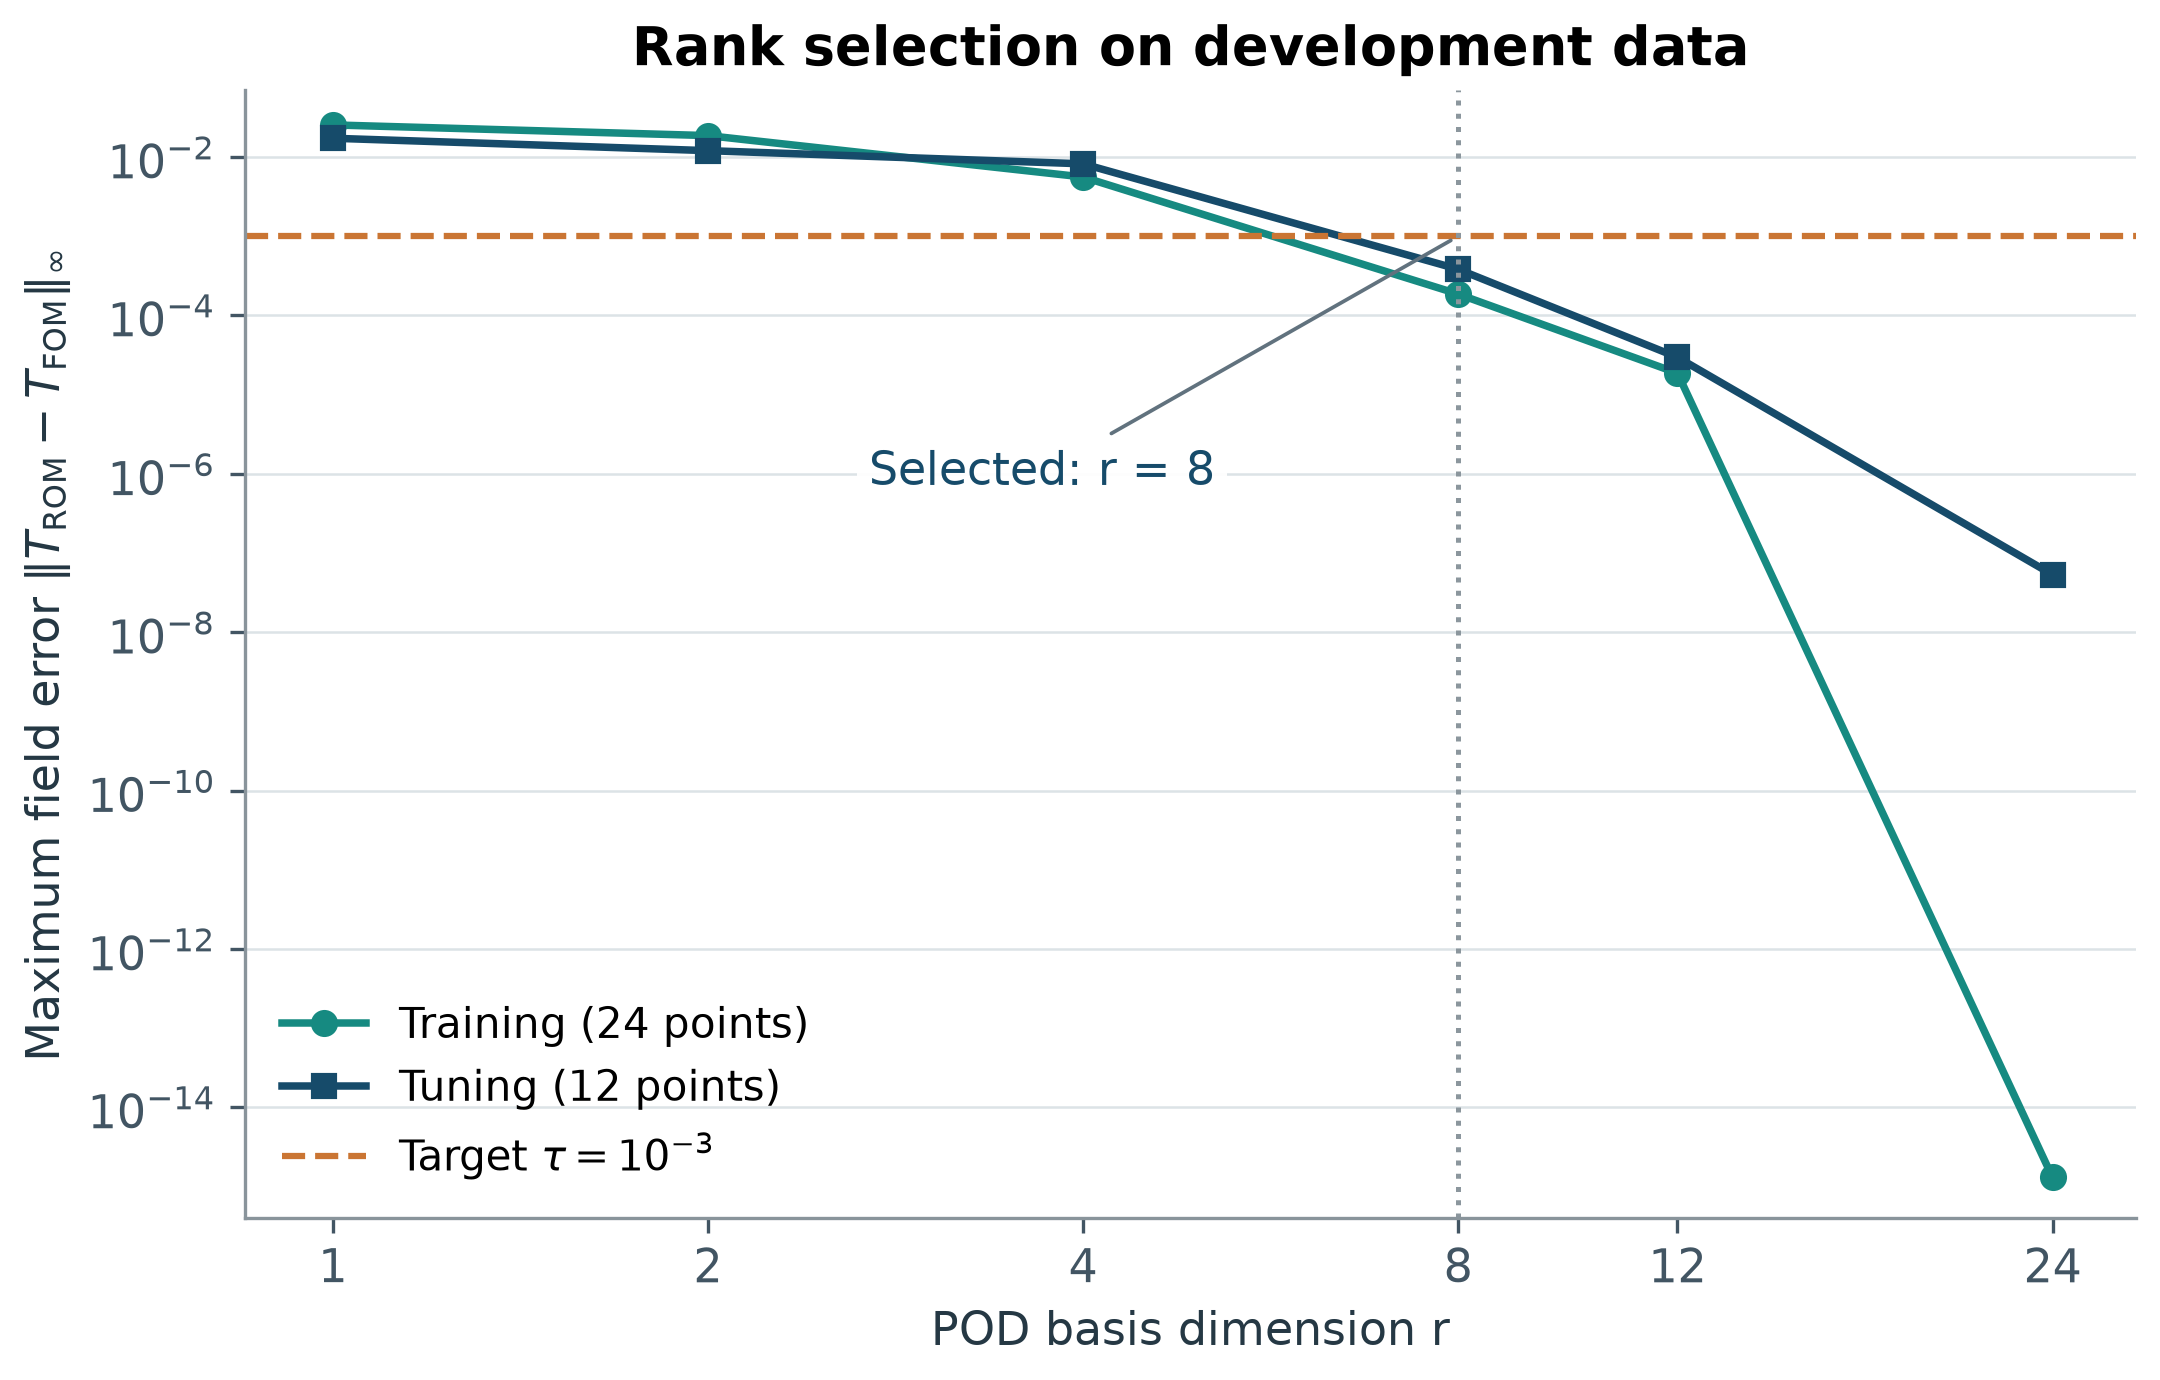
\includegraphics[width=0.78\linewidth,height=72mm,keepaspectratio]{figures/development_rank_curve.png}
\caption{开发数据上的选秩曲线；虚线为场误差目标 $10^{-3}$。}
\label{fig:development-rank}
\end{figure}

保持 $r=8$ 不变后，16 个边界角点中有 2 个\emph{场误差}超标：$\mu=(0.2,0.2,0.2,0.2)$ 的 $e_\infty=3.979763\times10^{-3}$，$\mu=(5,5,5,5)$ 的 $e_\infty=1.408608\times10^{-3}$。这两个点对应的热点值误差分别为 $4.033596\times10^{-4}$ 和 $2.081134\times10^{-4}$，均低于 $10^{-3}$；因此结论是场精度失效，不能改称热点值超标。最坏场误差案例见图~\ref{fig:development-fields}，误差较大区域与最高温位置并不一致。

\begin{figure}[htbp]
\centering
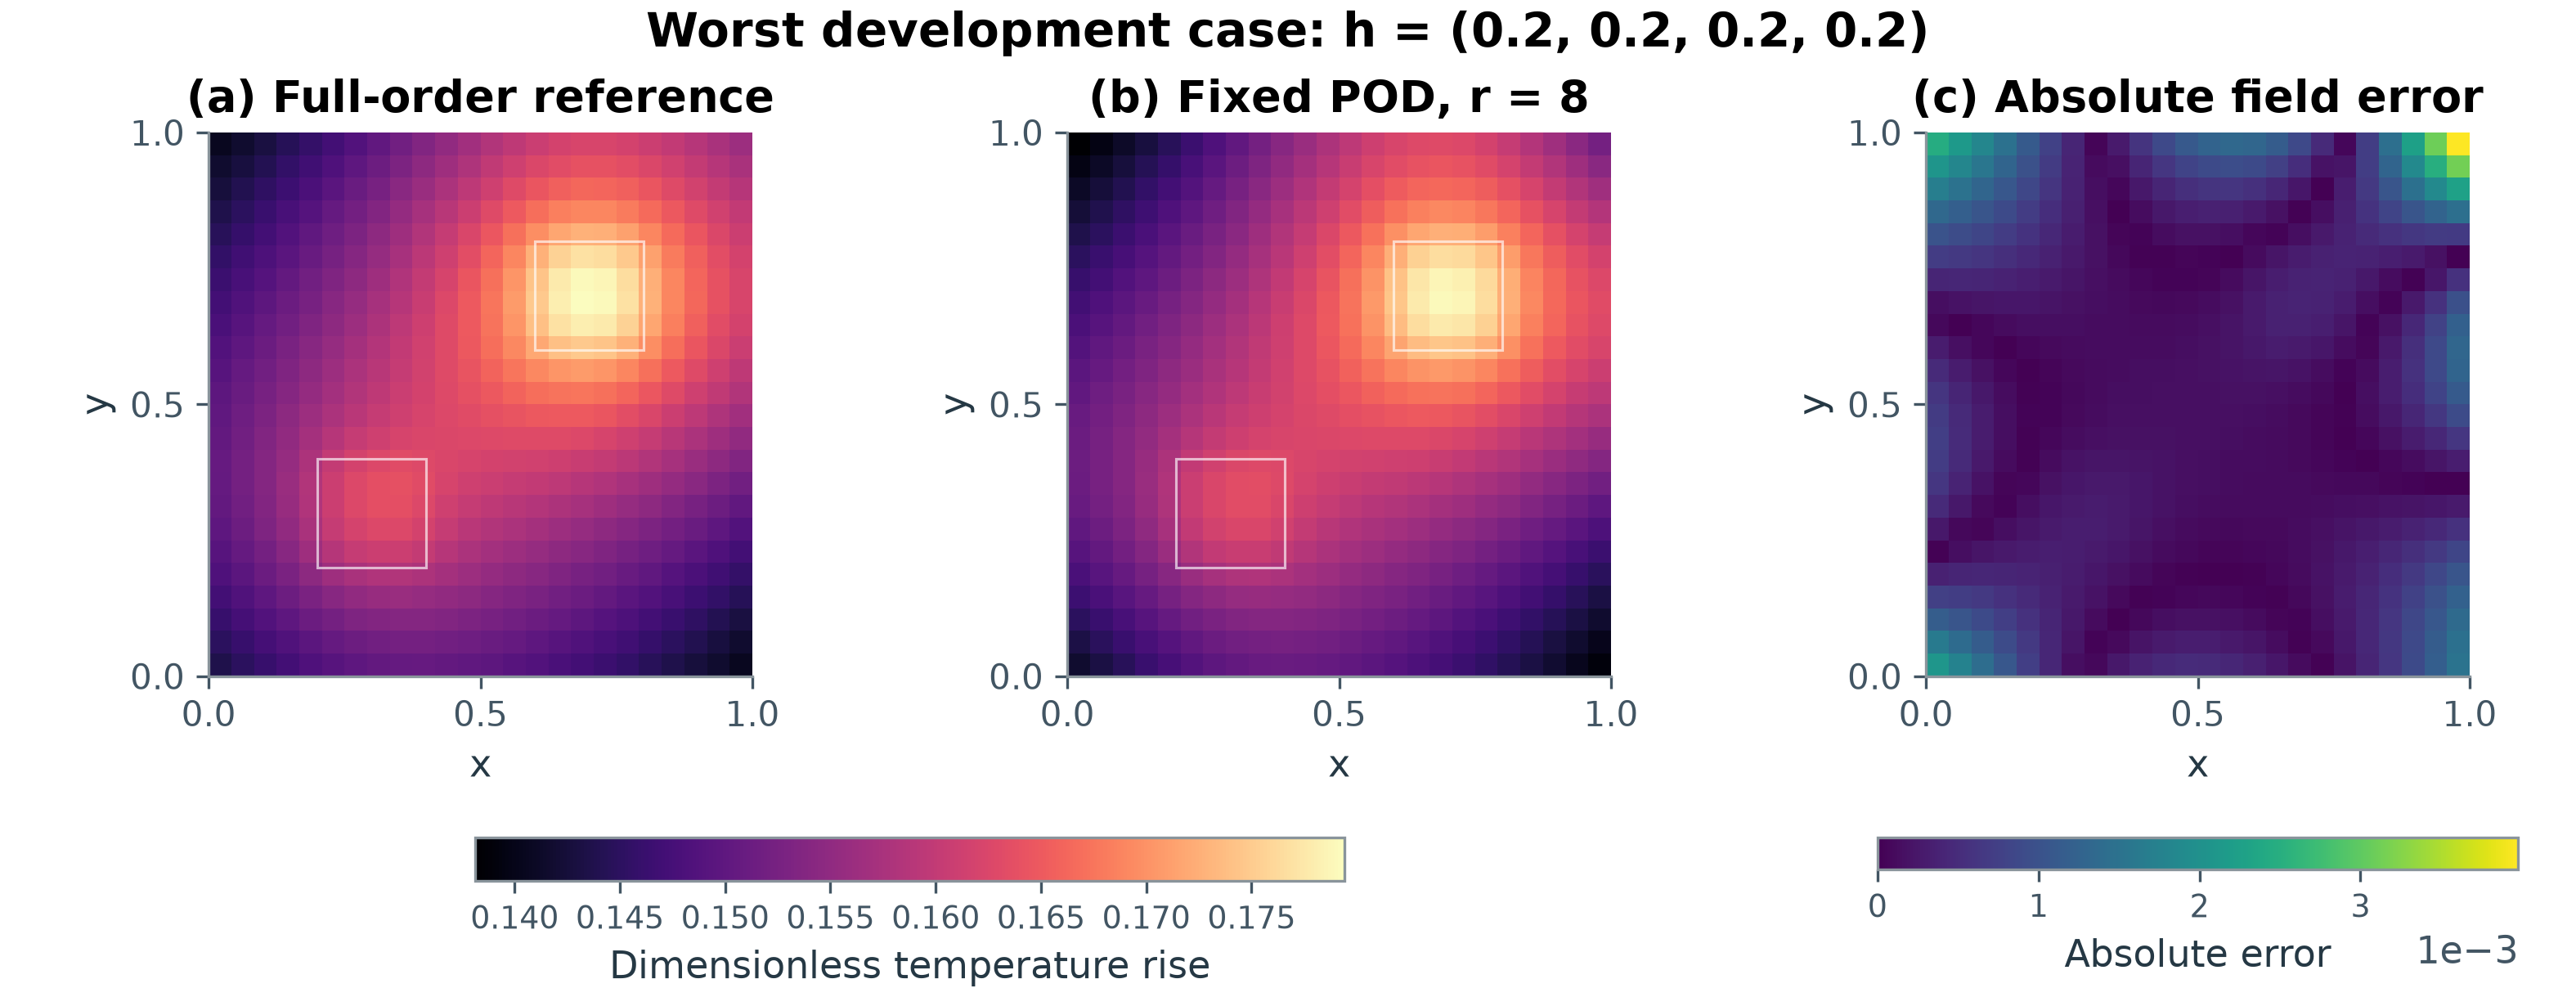
\includegraphics[width=\linewidth,height=64mm,keepaspectratio]{figures/development_worst_fields.png}
\caption{最坏开发案例的完整温度场、固定 POD 与逐点绝对误差。}
\label{fig:development-fields}
\end{figure}

\clearpage
\subsection{屏障覆盖误差，但预警明显保守}
阶段 3 复用 12 个调参案例，另执行 16 次 FOM 和 16 次 ROM，形成 28 个开发案例；没有在本阶段更新基。使用 $\eta>\tau$ 作为候选触发规则时，28 个案例都会触发，其中 2 个确实存在场误差超标，另外 26 个原近似已达到场误差目标。本组案例没有漏警，但不能据此推断任意浮点计算均无漏警。

效能比定义为 $\eta/e_\infty$。这 28 个案例的效能比范围为 $330.329$ 至 $734.112$，中位数为 $529.804$。最坏场误差点的 $\eta=1.417555$，约为实际误差的 $356.191$ 倍。图~\ref{fig:development-indicator} 表明，该界在当前样本上能覆盖误差，却可能引发大量额外完整求解。安全性、保守性和成本是需要同时研究的三个目标，不能只以覆盖误差宣称方法有效。

\begin{figure}[htbp]
\centering
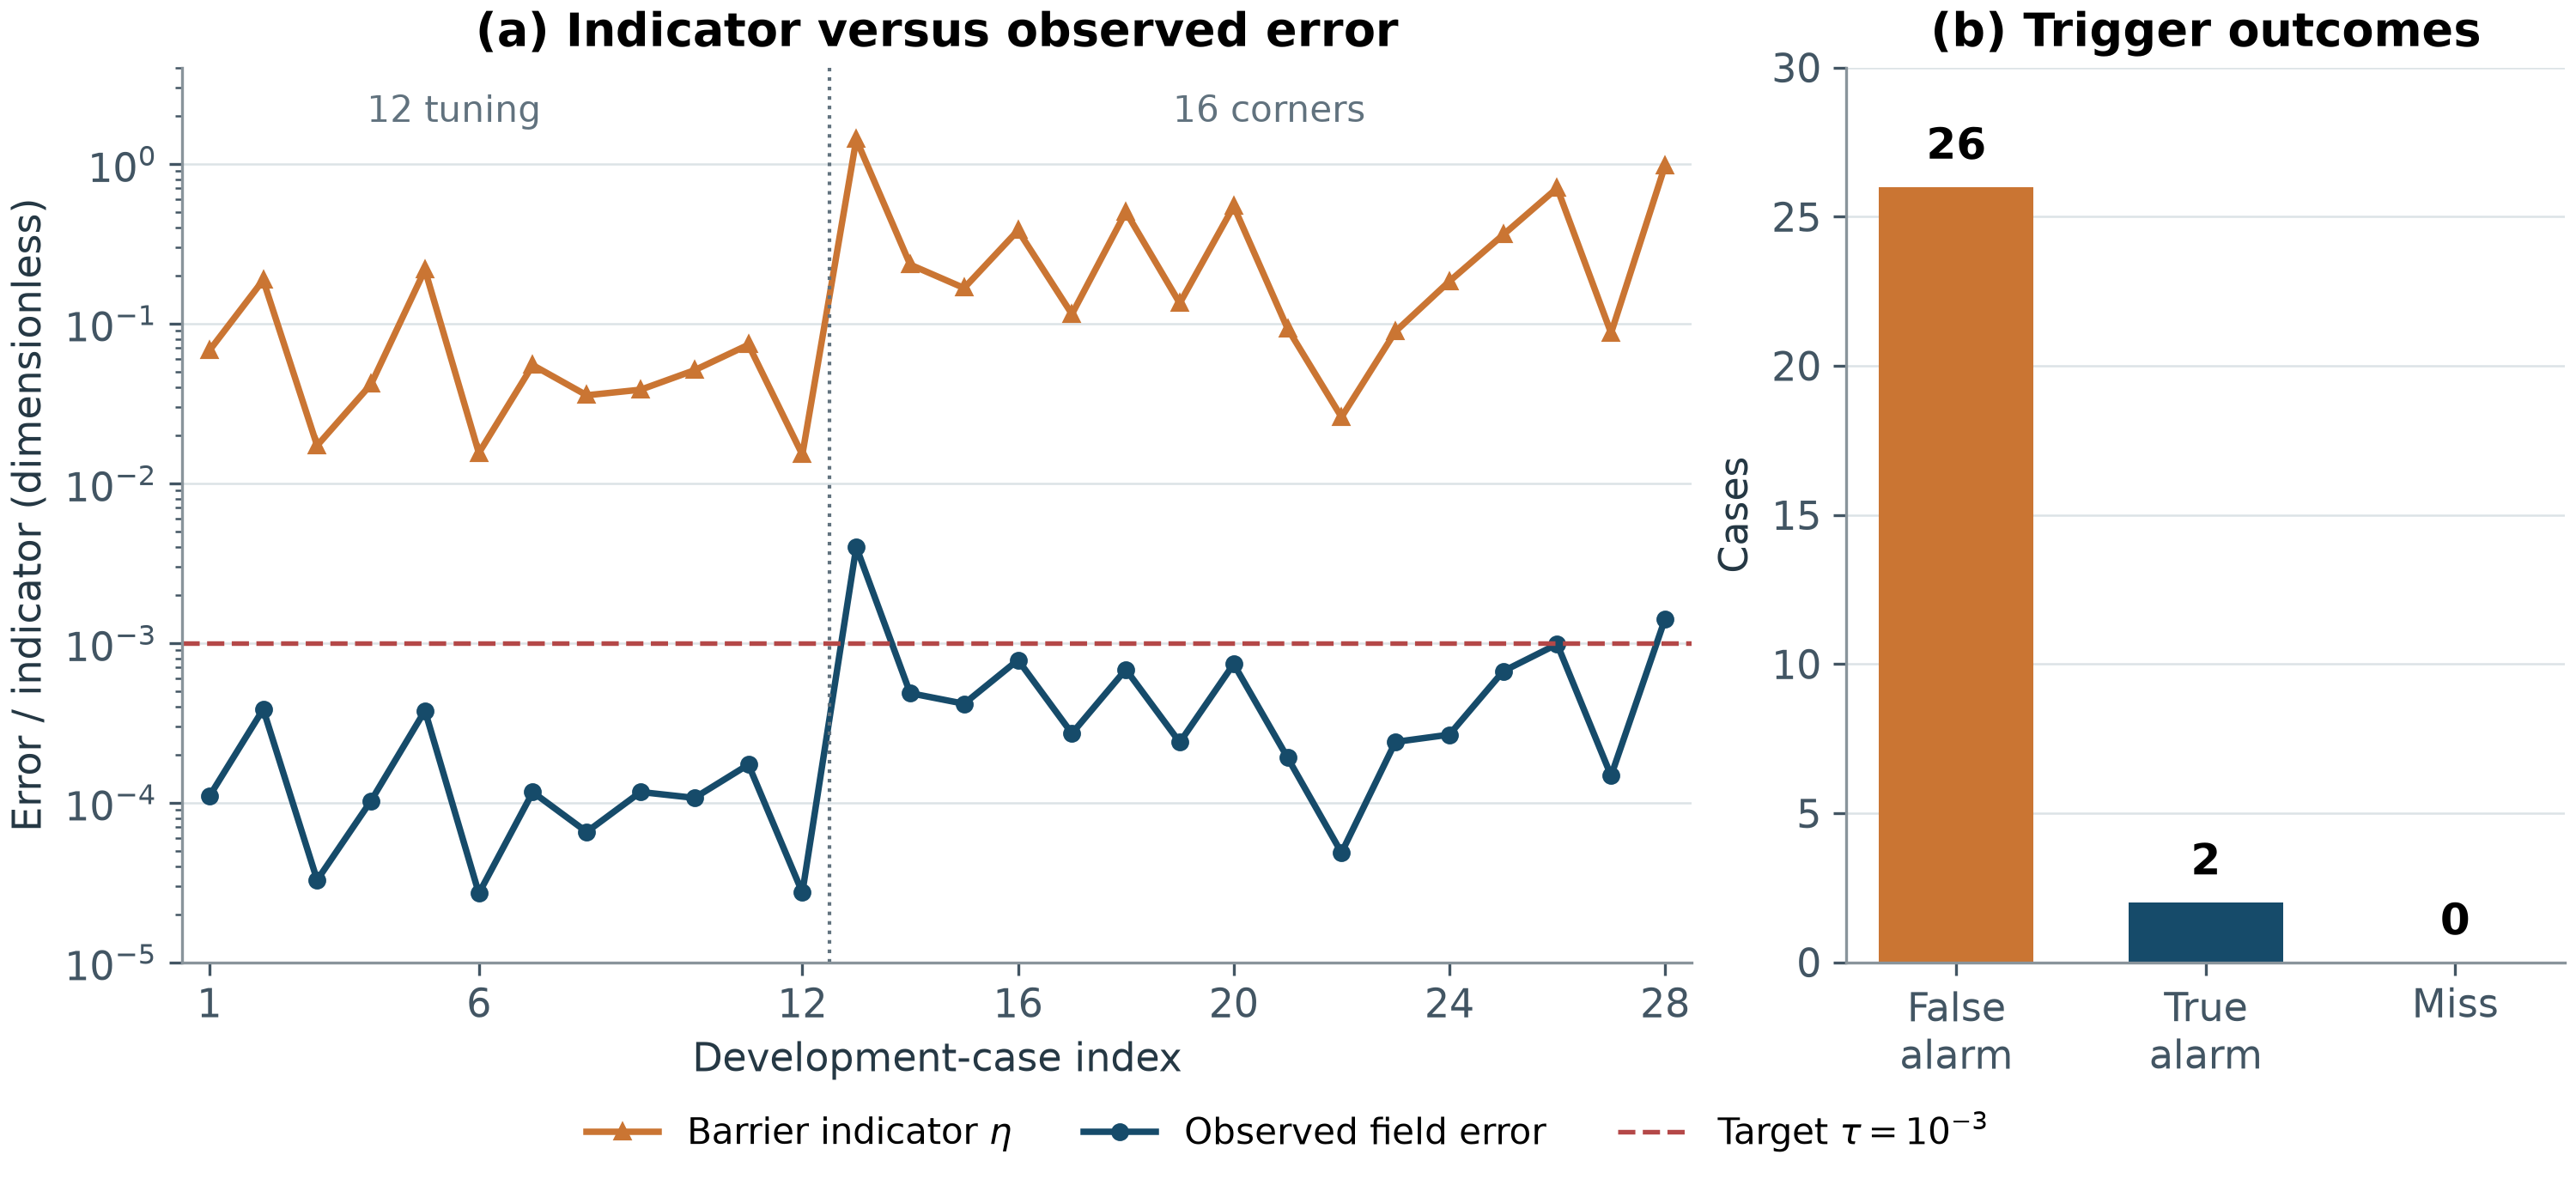
\includegraphics[width=\linewidth,height=75mm,keepaspectratio]{figures/development_indicator_failures.png}
\caption{28 个开发案例的屏障指标与实测场误差；右图按回退前误差统计候选触发。}
\label{fig:development-indicator}
\end{figure}

Moonshine 还以 \texttt{Fraction} 对 $n=1,2,3,4$ 的各 16 个参数角点作精确算术核对，共 64 组、480 个单元，均满足解析屏障不等式。普通双精度检查的最小 $(Az)_P$ 为 $0.9999999999995453$，与精确界的差异处于舍入量级；报告据此保留浮点评估与严格认证之间的区别。

\subsection{加入离线成本后，短批量尚未取得总体加速}
基线开发实现对每个参数重新装配完整矩阵，再投影、求解和重构。其 12 个调参查询的时间分解见表~\ref{tab:development-cost}。所选秩的在线时间比为
\[
 \frac{t_{\mathrm{FOM},12}}{t_{\mathrm{ROM,online},12}}
 =\frac{0.0241535}{0.0138724}\approx1.741.
\]
若按“训练快照、SVD、所选秩的 12 次查询”的部署成本口径，将一次离线成本完整计入，则
\[
 \frac{t_{\mathrm{FOM},12}}
 {t_{\mathrm{snapshot}}+t_{\mathrm{SVD}}+t_{\mathrm{ROM,online},12}}
 =\frac{0.0241535}{0.0677765}\approx0.356.
\]
后一比值小于 1，表示这个短批量下的直接完整求解更省时。不能把 $1.741$ 写成含离线成本的总加速倍数。

\begin{table}[htbp]
\centering
\caption{12 个调参查询的开发阶段时间分解（秒）}
\label{tab:development-cost}
\small
\begin{tabular}{lr}
\toprule
项目 & 实测时间 \\
\midrule
24 个训练快照的离线计算 & 0.0504288 \\
SVD 建基 & 0.0034753 \\
所选 $r=8$ 的 12 次 ROM 在线计算 & 0.0138724 \\
上述离线与在线之和 & 0.0677765 \\
12 次 FOM 组装与求解 & 0.0241535 \\
\bottomrule
\end{tabular}
\end{table}

这些时间来自单次开发观测，存在计时噪声，而且 ROM 在线计时含残差评估，FOM 对照未含另外记录的残差时间，故尚不是统一输出服务下的最终性能基准。上述部署成本也不包括全部选秩搜索、调参与文件保存等研究开销；这些开销保存在原始记录中，没有被宣称为零。开发结果提出了后续比较的具体要求：复用组装结构、设置快速 FOM 对照、统一计时边界，并检验不同查询批量下离线成本能否摊销。

\subsection{外部复算与证据对应}
三份外部复核分别完成 84 组矩阵与源装配对照、36 次 FOM 与 216 次 ROM 复算，以及全部 28 个失效开发案例的 FOM/ROM 复算。基线复算的最大场数组差不超过 $4.025\times10^{-16}$；失效分析的场误差指标差不超过 $5.552\times10^{-17}$，效能比与 $28/2/26$ 触发统计均得到复现。原生的 64 组有理数检查也与外部精确计算一致。以上次数与 Moonshine 原生执行分别记账，不能相加后声称全部由同一智能体自主完成。

数值来源为 \texttt{workspace/results/01\_model.json}、\texttt{02\_baseline.json} 和 \texttt{03\_failure.json}；外部复核依据为 \texttt{independent\_review/stage01\_crosscheck.json}、\texttt{stage02\_crosscheck.json}、\texttt{stage03\_crosscheck.json}。审核状态以原版事件记录为准：早期产物中的“待审核”字段保留其生成时状态，不用事后修改覆盖失败或未定记录。

\section{改进算法与独立评价协议}
\subsection{快速组装与自适应回退}
固定网格与热源后，几何项 $K,D_s,b$ 可以预存。完整模型的公平快速对照每次只更新四个边界系数，然后仍完整求解同一稀疏线性系统。降阶模型则预存
\[
 K_r=V^\top KV,\qquad D_{r,s}=V^\top D_sV,\qquad b_r=V^\top b,
\]
在线求解 $(K_r+\sum_s\beta_sD_{r,s})a=b_r$，再重构完整温度场 $Va$。参数分离属于标准投影降阶技术，本研究的贡献是可核查的实现、失效分析与成本比较，不宣称这一公式的新颖性。

自适应模型先作快速降阶预测 $u_r$，再计算积分方程残差 $b-Au_r$ 及解析屏障指标 $\eta$。若 $\eta\leq\tau$，返回预测场；否则\textbf{实际执行}快速完整求解并返回其结果。回退解随后作两遍整体正交投影消去，即两遍重正交（CGS2）；当其剩余二范数与完整解二范数之比大于 $10^{-10}$、当前秩小于 $\min(32,n^2)$ 时，加入归一化剩余向量并更新全部低维缓存。达到秩上限或向量相关时仍执行所需回退，但不增广。零解不增广，域外参数及非有限数值被拒绝。

原生开发程序执行了 653 项检查：原与快速完整模型、原与快速投影的一致性，残差和正交性，触发规则，以及零向量、相关向量、非法参数和最小网格等分支均通过。52 个开发参数上的两种完整解之差为零，两种固定降阶场的最大差为 $7.49\times10^{-16}$。按 12 个调参案例再接 16 个边界角点的顺序运行时，发生 15 次真实回退及增广，秩由 8 增至 23；这 15 次均属于回退前近似已达标的保守触发。该结果仅作开发证据，不能当作独立测试表现。

\subsection{测试隔离与五种对照}
评价协议在最终测试生成前固定：每边网格数 $n\in\{24,48,96\}$，每个网格沿用相同的 24 个训练参数、重新计算对应网格上的训练解与奇异值分解。初始秩统一使用开发阶段选定的 $r=8$，不再根据最终测试调秩。测试包含 256 个按既定顺序使用的参数，随机种子为 20261027，各分量在 $[0.2,5]$ 内独立对数均匀采样。采样前保存算法、驱动与配置的摘要；模型函数不能取得用于事后评价的参照解。

比较五种方法：原始完整组装 FOM、预存几何的快速 FOM、完整组装再投影的固定 POD、预存低维矩阵的快速固定 POD，以及带屏障触发和基更新的自适应 POD。\textbf{主要速度对照使用快速 FOM}，以免把消除 Python 组装开销误算成降阶本身的收益。各方法均返回完整温度场，固定 POD 与自适应 POD 使用同一初始基，以区分组装优化和误差控制的作用。

场误差定义为 $\|u-u_{\mathrm{FOM}}\|_\infty$，热点值误差定义为 $|\max u-\max u_{\mathrm{FOM}}|$，并另记录相对二范数误差。误触发严格定义为 $\eta>\tau$ 且\emph{回退前}场误差不超过 $\tau$；不能用回退后接近零的误差判断。普通双精度计算的指标不具备区间运算的向外舍入保证，报告将精确算术误差界与实际浮点观测分开陈述。

\subsection{完整成本与来源归属}
对查询数量 $Q\in\{24,256\}$，定义每种独立部署方案的总成本
\[
 C_m(Q)=C_{m,\mathrm{offline}}+\sum_{i=1}^{Q}t_{m,i},
 \qquad S_m(Q)=\frac{C_{\mathrm{fast\ FOM}}(Q)}{C_m(Q)}.
\]
只有 $S_m>1$ 才代表该口径下的总成本降低。离线成本按方法的实际需要归属：原始 FOM 不承担训练或 SVD；快速 FOM 承担所需几何和源项预处理；各 POD 方案承担 24 次训练求解、SVD 与初始基准备，快速及自适应方案另计所需投影缓存，自适应方案还计屏障准备。每个网格、每次计时重复中可以只实际执行一次共享训练与 SVD，再复制同一初始基供对照，但在每种独立部署的 ROM 成本账上均完整计入一次。\emph{实际实验调用总数不因此乘以方案数量}。短批量也承担全部必要离线成本。自适应在线服务时间包含残差与指标、触发后的真实完整求解、重正交及缓存更新。普通 FOM 和固定 POD 不强制承担可选残差诊断，其诊断成本单列；事后误差评价不计入服务时间。

评价预定每个网格做三次计时重复，逐次重建训练解并重置基、缓存、状态与计数；实际完成次数以结果文件为准。重复使用同一冻结参数序列，是时间波动观测，不是新增独立精度样本。程序在导入数值库前将相关线程环境变量设为 1，但这本身不是对底层实际线程数的独立测量；环境设置与计时范围保存在产物中。数值服务时间也不包含大模型思考、工具调度和人工复核时间；后者属于研究开发成本，不应隐去或混作数值加速。

研究求解器、快速组装内核及自适应策略实现由原版 Moonshine 的工具调用生成并迭代；最终采样、计时、记账与结果汇总驱动由外部协调者提供，另行记录来源及摘要，再交 Moonshine 审阅与执行。独立数学检查、图表和报告整理同样属于外部复核与呈现。文件被复制到智能体工作目录，不改变其作者归属。

\section{最终实验结果与结论}
\subsection{冻结参数流上的精度与触发行为}
最终汇总记录完成了三个网格、每个网格三次重复，共九次有效运行，缺失及无效运行数均为零。每次重复使用同一冻结的 256 个参数；下列精度和轨迹在三次重复中一致，因此每个网格的精度样本量仍为 256，而不是 768。前 24 次查询只是同一序列的前缀，不是另一组测试。这些参数未参与初始建模与选秩；自适应评价则允许按顺序使用当前已付费执行的 FOM 回退解更新基，并将状态传给后续查询。它属于在线顺序评价，不是全程冻结模型的测试；每次计时重复重置全部学习状态，事后参照真解不作为免费预测接口。

\begin{table}[htbp]
\centering\small
\caption{256 次查询的实际输出误差。固定模型使用快速 $r=8$ POD；超标阈值为 $10^{-3}$。}
\label{tab:final-accuracy}
\begin{tabular}{rlrrrr}
\toprule
$n$ & 方法 & 最大场误差 & 最大热点值误差 & 场超标数 & 热点超标数\\
\midrule
24 & 固定 POD & $1.972\times10^{-3}$ & $1.453\times10^{-4}$ & 6 & 0\\
24 & 自适应 POD & $1.270\times10^{-6}$ & $1.132\times10^{-8}$ & 0 & 0\\
48 & 固定 POD & $2.211\times10^{-3}$ & $1.471\times10^{-4}$ & 6 & 0\\
48 & 自适应 POD & $2.967\times10^{-7}$ & $1.043\times10^{-9}$ & 0 & 0\\
96 & 固定 POD & $2.342\times10^{-3}$ & $1.470\times10^{-4}$ & 7 & 0\\
96 & 自适应 POD & $1.203\times10^{-7}$ & $7.415\times10^{-10}$ & 0 & 0\\
\bottomrule
\end{tabular}
\end{table}

完整组装与快速固定 POD 的误差仅有浮点量级差异，场超标计数相同。表\ref{tab:final-accuracy}说明，仅监测热点值会遗漏本次出现的温度场失准。自适应方案在这些有限测试上均达标，但其触发质量必须单独评价：三个网格分别触发 15、15、17 次实际 FOM 回退，全部成功增广，最终秩分别为 23、23、25；这 47 次触发的\textbf{当前回退前 ROM 场误差均已达标}，因此全部属于按既定定义统计的误触发。不存在漏报的观测也不能证明判别器最优。较保守的触发提前增加了基向量，后续精度改善伴随这些基更新出现，不能把每次触发描述为发现了真实超标。

\begin{figure}[htbp]
\centering
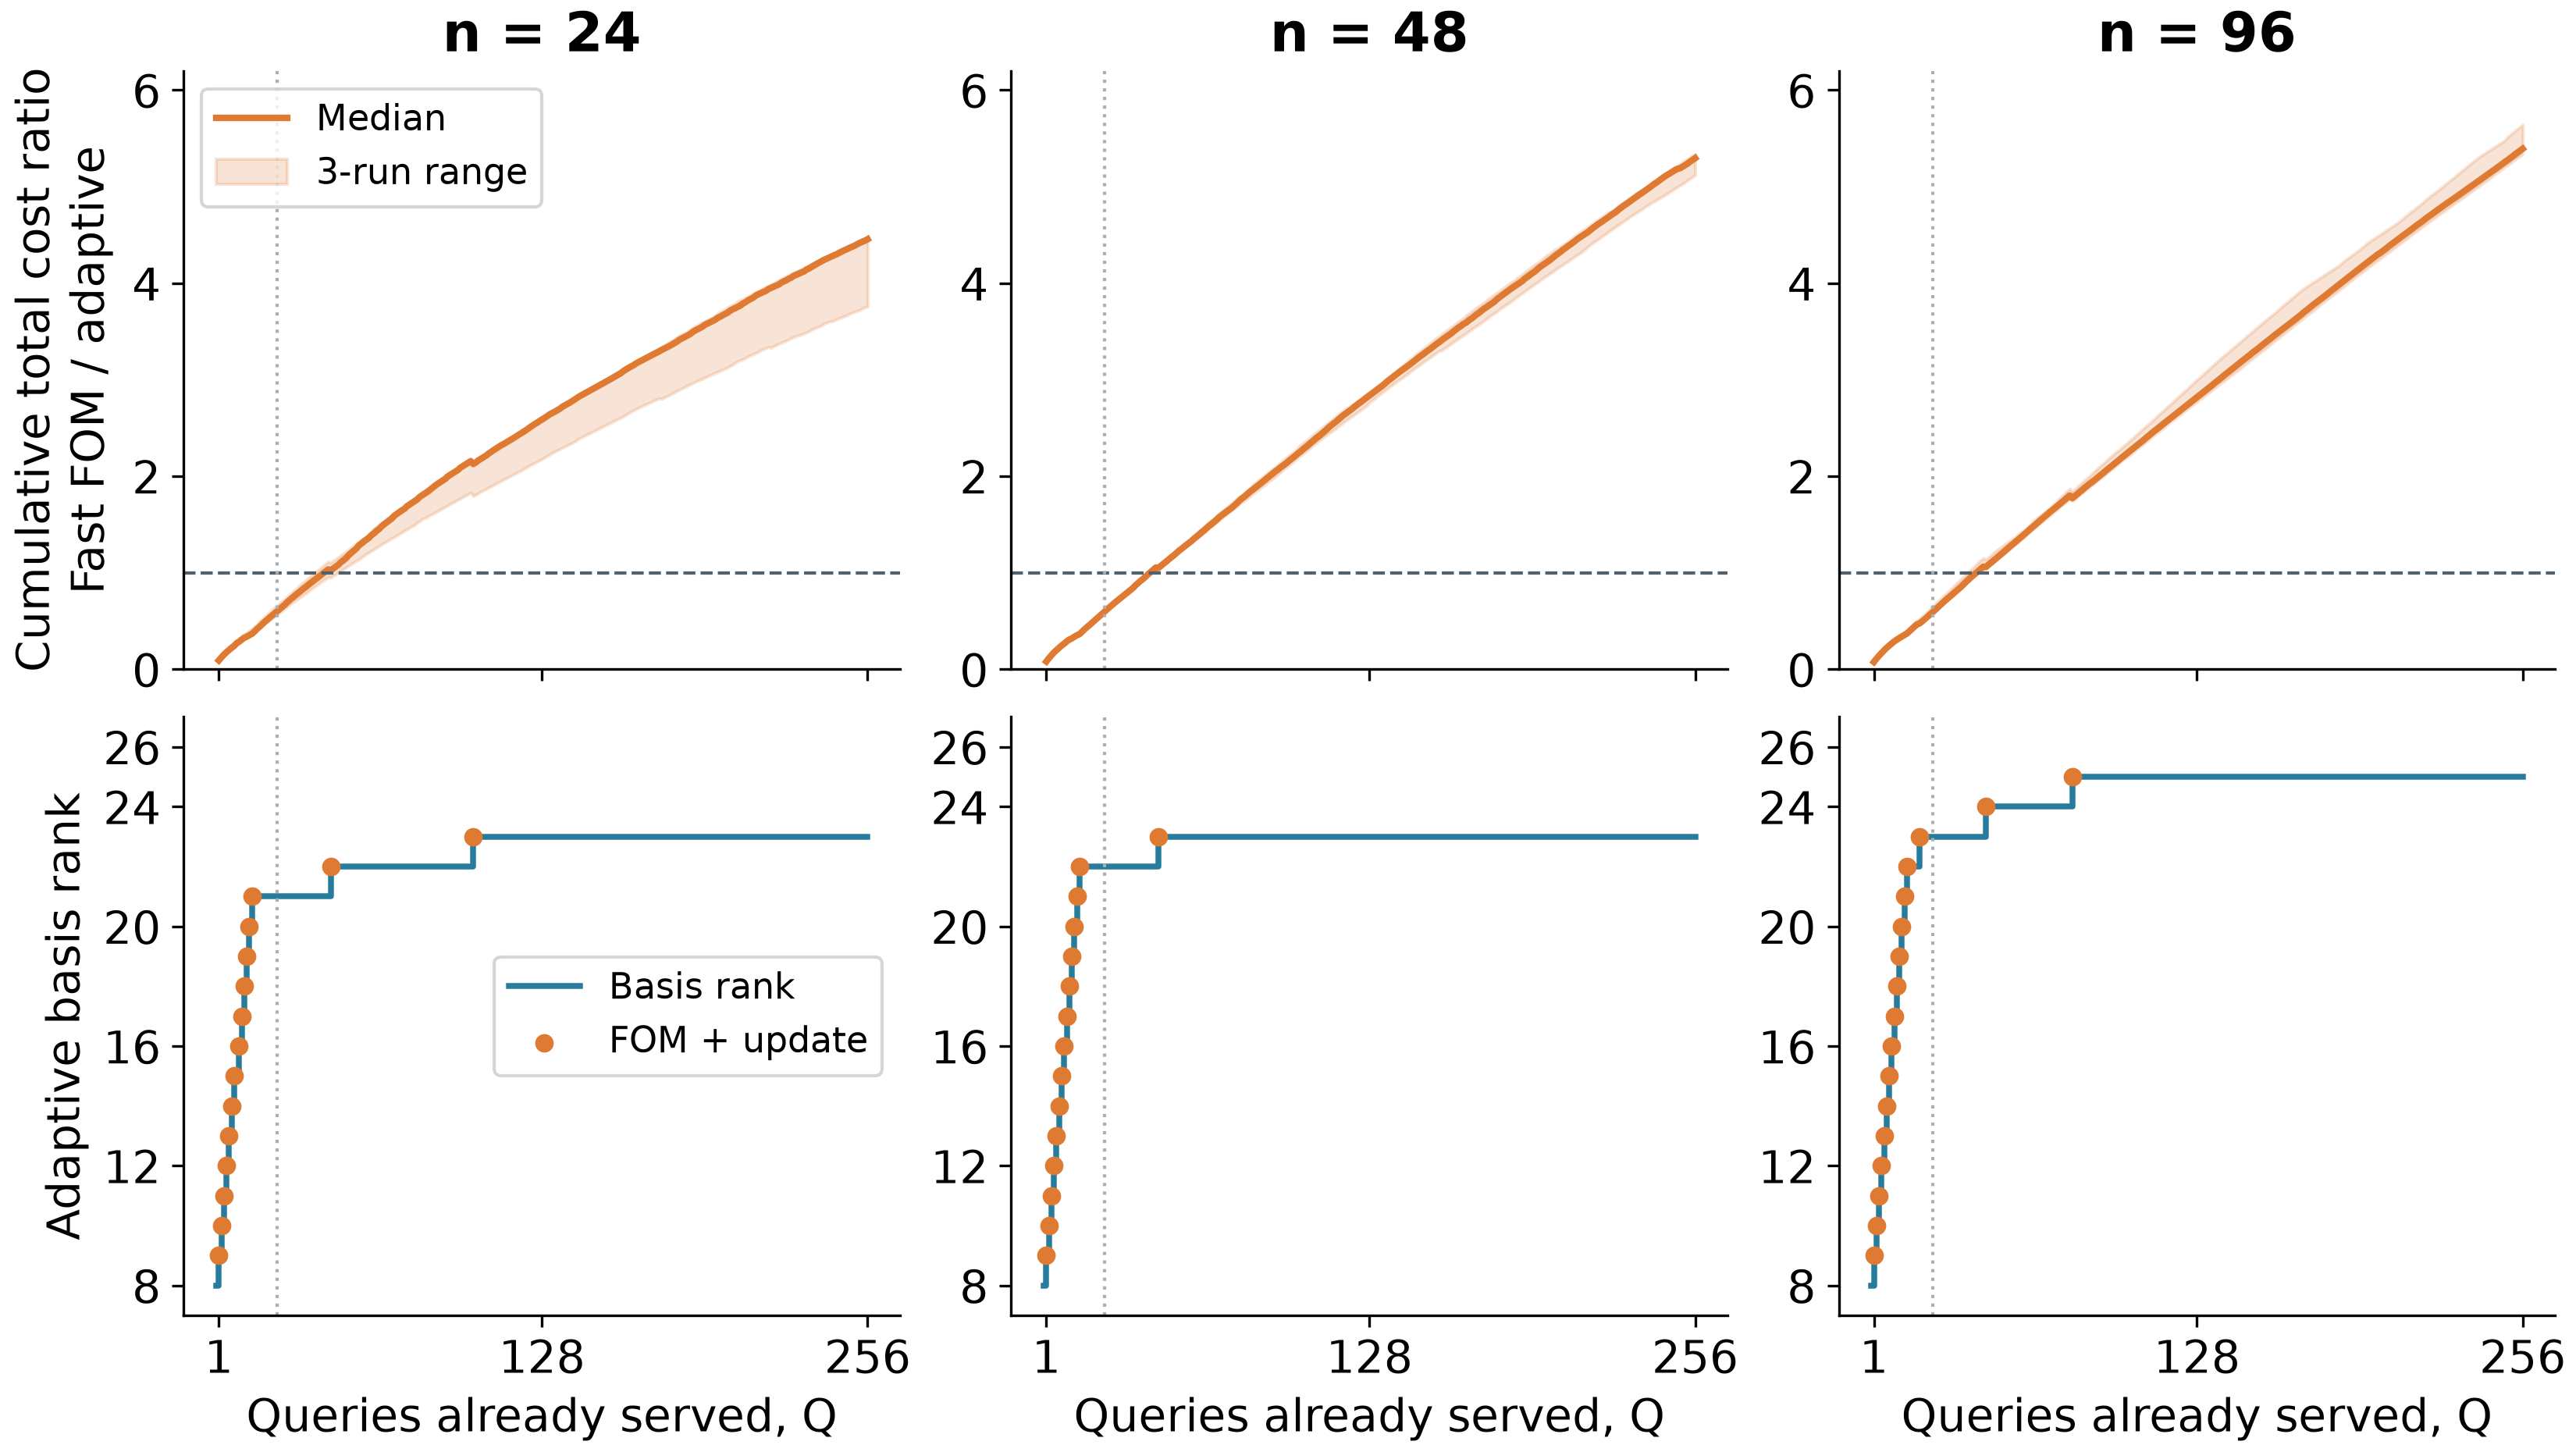
\includegraphics[width=0.94\linewidth]{figures/final_online_trace.png}
\caption{冻结参数流上的累计总成本比与基更新轨迹。阴影为三次计时的最小--最大范围，不是置信区间；竖虚线表示第 24 次查询。基更新轨迹在重复运行中一致。触发标记对应回退前的屏障判断，不能将回退后的误差当作触发准确性的依据。}
\label{fig:final-trace}
\end{figure}

\subsection{计入离线投入后的成本}
表\ref{tab:final-cost}使用前节定义的必要部署成本 $C_m$，以及以快速 FOM 为分子的总成本比 $S_m$。各列分别取三次重复的中位数；比值是\emph{逐次配对计算后再取中位数}，不要求等于两个耗时中位数的商。表内秒数不包含大模型研究、人工复核、报告制作和可选事后诊断。

\begin{table}[htbp]
\centering\small
\caption{五种方法的必要总成本（秒）及配对成本比中位数。$S>1$ 表示比快速 FOM 节省总成本。}
\label{tab:final-cost}
\begin{tabular}{rlrrrr}
\toprule
 & & \multicolumn{2}{c}{$Q=24$} & \multicolumn{2}{c}{$Q=256$}\\
\cmidrule(lr){3-4}\cmidrule(lr){5-6}
$n$ & 方法 & $C_m$ & $S_m$ & $C_m$ & $S_m$\\
\midrule
24 & 原始 FOM & 0.045281 & 0.456 & 0.508565 & 0.393\\
24 & 快速 FOM & 0.021096 & 1.000 & 0.201588 & 1.000\\
24 & 原始固定 POD & 0.047435 & 0.426 & 0.304257 & 0.666\\
24 & 快速固定 POD & 0.019477 & 1.004 & 0.023815 & 8.561\\
24 & 自适应 POD & 0.032453 & 0.603 & 0.045845 & 4.455\\
\midrule
48 & 原始 FOM & 0.171587 & 0.403 & 1.820013 & 0.395\\
48 & 快速 FOM & 0.069271 & 1.000 & 0.719447 & 1.000\\
48 & 原始固定 POD & 0.177342 & 0.398 & 1.166352 & 0.611\\
48 & 快速固定 POD & 0.071240 & 0.972 & 0.076377 & 9.304\\
48 & 自适应 POD & 0.115201 & 0.600 & 0.135209 & 5.295\\
\midrule
96 & 原始 FOM & 0.748842 & 0.460 & 8.197976 & 0.439\\
96 & 快速 FOM & 0.344734 & 1.000 & 3.543090 & 1.000\\
96 & 原始固定 POD & 0.763728 & 0.451 & 4.702765 & 0.753\\
96 & 快速固定 POD & 0.355942 & 0.969 & 0.363834 & 9.738\\
96 & 自适应 POD & 0.585963 & 0.588 & 0.657066 & 5.392\\
\bottomrule
\end{tabular}
\end{table}

\begin{table}[htbp]
\centering\small
\caption{自适应方案总成本比：中位数及三次计时的最小--最大范围。范围不是置信区间。}
\label{tab:final-ranges}
\begin{tabular}{rcc}
\toprule
$n$ & $Q=24$ & $Q=256$\\
\midrule
24 & $0.602599\;[0.570927,\,0.662752]$ & $4.455223\;[3.759159,\,4.461084]$\\
48 & $0.599792\;[0.599714,\,0.602662]$ & $5.294642\;[5.117985,\,5.339706]$\\
96 & $0.588320\;[0.579459,\,0.648001]$ & $5.392289\;[5.335244,\,5.640081]$\\
\bottomrule
\end{tabular}
\end{table}

短批量 $Q=24$ 时，自适应方案在三个网格上均未摊平离线成本；不能以在线服务加速替代这一结论。$Q=256$ 时，总成本比中位数约为 $4.46$--$5.39$，同时保持本次所有返回场达标。快速固定 $r=8$ POD 更省时，但存在场超标。原始固定 POD 的总成本比始终低于 1，说明低维求解本身不足以抵消重复组装与投影的开销。

\begin{figure}[htbp]
\centering
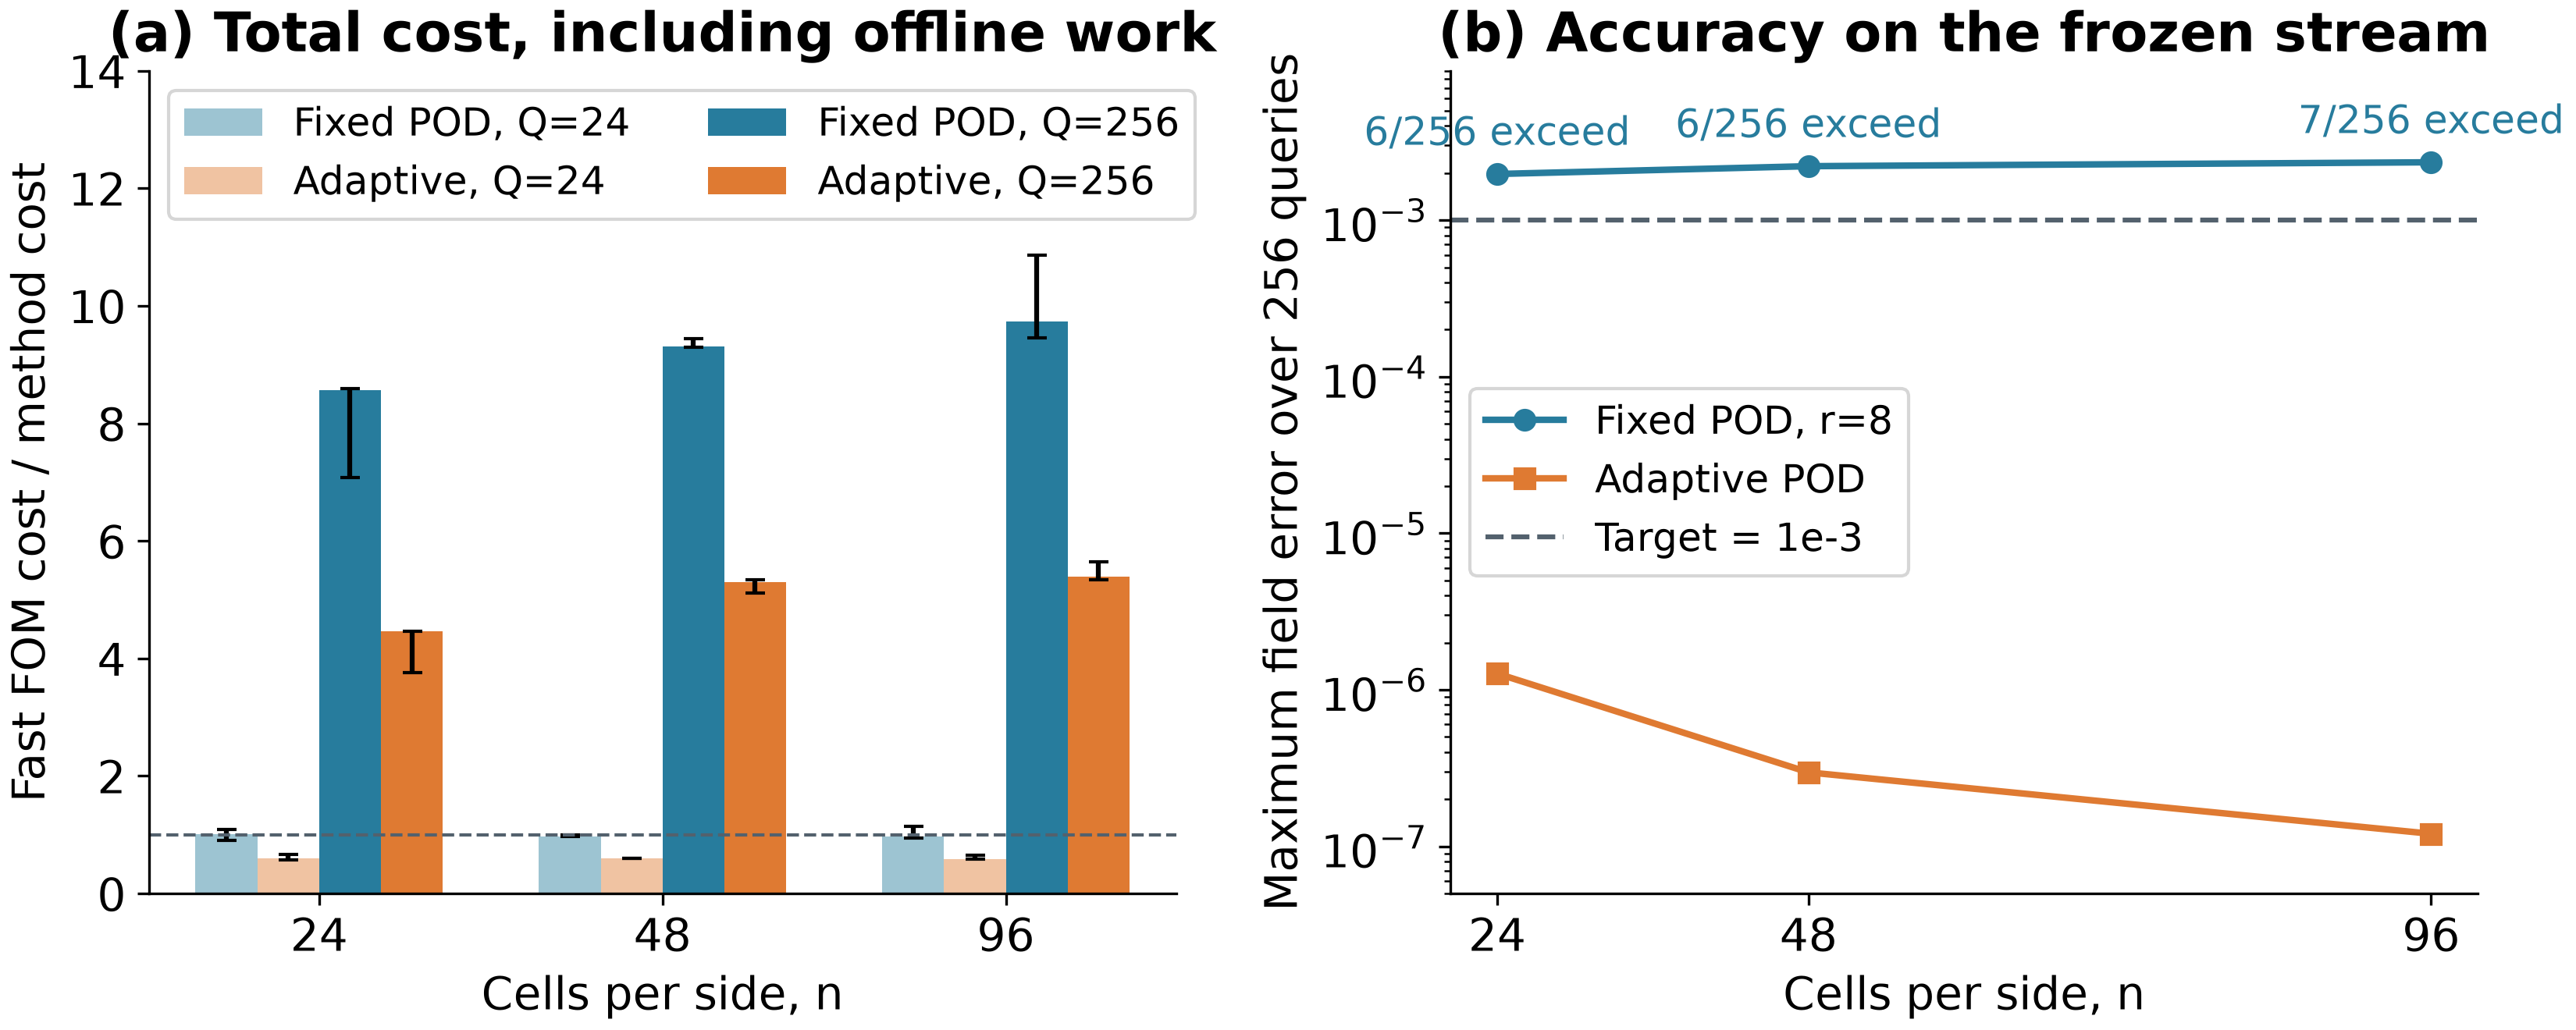
\includegraphics[width=0.94\linewidth]{figures/final_cost_accuracy.png}
\caption{最终精度与完整成本的联合比较。计时汇总基于同一参数序列的三次重复；所示最小--最大范围仅表示本机计时波动，不是置信区间，也不是新增精度样本。}
\label{fig:final-cost}
\end{figure}

运行环境为 Windows、Intel Core Ultra 9 275HX、约 63.38 GiB 内存，Python 3.12.14、NumPy 2.3.5、SciPy 1.18.1。线程环境变量请求单线程，但底层实际线程池规模未独立测量；桌面后台负载也未完全隔离。因此这些秒数和范围属于本机观测，不能外推为跨硬件性能保证。

\subsection{独立复核、完成范围与后续问题}
外部复核记录 \texttt{final\_crosscheck.json} 的 24 项检查全部通过，包含冻结顺序与摘要、九次运行及汇总记账、原生执行证据和独立数值复算。外部实际另做了 72 次训练 FOM、768 次参照 FOM、768 次固定 ROM、768 次自适应 ROM 及 47 次回退，按三个网格各复放一次相同参数流；这些工作不计入 Moonshine 原生调用次数或部署成本，也没有产生新的测试参数。场误差统计最大差为 $3.63\times10^{-15}$ 以下，指标差为 $2.81\times10^{-12}$ 以下，保存的最坏温度场差为 $3.56\times10^{-15}$ 以下。原生文件摘要保持不变。该复核是普通浮点程序证据，不是区间认证或形式化证明。

最终结果首次提交 Moonshine 审核时，计算与逻辑审核为正确，假设审核因材料未展开两个矩形热源的单元面积积分式而未能确定，整体未通过。后续补充源项定义及总热量 $\sum b_{ij}=0.12$ 后，原生综合审核通过；补证未改变算法、测试参数或数值结果，首次未定记录仍保留。该模型审核与外部程序复算是两条不同的证据链，均不能冒称形式化数学证明。

本研究已形成从离散模型、固定 POD 失效、解析屏障检查，到真实回退与基更新、冻结测试和成本复核的可追溯数值闭环。在本次有限合成参数流上，自适应方案以一定额外开销换取了较小的场误差，并在长查询批量中摊平离线投入；短批量失败和全部保守触发同样是研究结果。\textbf{最终协议没有比较固定 $r=24$ 等更强基线}，尽管已有 24 个训练快照，因此不能声称优于最优固定 ROM，也不能把本实验提升为工业热仿真问题已经解决。

下一步可检验的问题是：在同一独立部署成本和新增冻结测试下，增加固定基维数与收紧屏障估计，哪一种更有效地减少误触发和总耗时？连续 PDE 的离散误差、三维复杂结构、温度相关材料和非线性边界仍在本研究范围之外。解析屏障依托已有单调矩阵思想，由外部先验提供、经 Moonshine 检查和实现；本项目的价值在于实际研究过程及其可核验边界，而非宣称发现新的通用定理。

\section{真实研究迭代与证据核验}
\subsection{七轮研究的运行轨迹}
表~\ref{tab:research-turns} 根据原版事件、逐轮摘要及最终外部审计形成，覆盖 2026 年 10 月 25 日完成的七个研究轮次。单次研究轮次可包含多个子任务，也可能失败；不能将“四阶段菜单”理解为四次调用就完成研究。

\begin{table}[htbp]
\centering
\caption{七轮研究证据；时间为当日日本时间，调用列为接受数/失败数}
\label{tab:research-turns}
\small
\setlength{\tabcolsep}{4pt}
\begin{tabular}{clrrrrp{0.22\linewidth}}
\toprule
轮次 & 时间与主要任务 & 调用 & Python 成功 & 审核通过 & 归档 & 状态 \\
\midrule
1 & 15:44 建模校验 & 9/1 & 3 & 0 & 8 & 局部未完成 \\
2 & 16:02 补证复核 & 15/0 & 1 & 1 & 5 & 局部闭环完整 \\
3 & 16:23 POD 与失效分析 & 13/0 & 2 & 1 & 3 & 局部闭环完整 \\
4 & 16:47 改进首次尝试 & 2/1 & 0 & 0 & 4 & 模型请求超时 \\
5 & 16:56 改进内核开发 & 13/0 & 1 & 1 & 4 & 局部闭环完整 \\
6 & 17:31 冻结最终评价 & 13/0 & 7 & 0 & 7 & 实验完成，审核材料未充分 \\
7 & 17:53 热源补证复审 & 12/0 & 1 & 1 & 7 & 局部闭环完整 \\
\midrule
合计 & 全部已结束轮次 & 77/2 & 15 & 4 & 38 & 4 个局部闭环完整 \\
\bottomrule
\end{tabular}
\end{table}

“调用”是本地 Provider 的预约及响应记录，不是服务端重试次数或精确计费请求数。Python 成功表示原版工具实际返回退出码 0，不表示相同数量的新数学定理；共 16 次 Python 工具尝试中有 15 次成功。审核列统计整体审核通过的次数；归档条目可包含计划、失败和局部结论，不能仅凭存在归档判断研究完成。共 6 次整体审核尝试，其中 2 次因材料不足未定、4 次通过。38 条归档均与原版研究记忆匹配。

七轮记录的配置模型均为 \texttt{gpt-6-astra}。假设、计算、逻辑三个维度是该配置下具有不同审核职责的模型调用，不是三个互相独立的数学证明。文中的“外部独立复核”则指另外实现的组装、程序、推导和复算证据，两者不能混称。

七轮墙钟耗时之和为 $7407.187$ 秒，约 $123.45$ 分钟，包括模型等待、工具运行与原版审核归档，但不包括轮间协调、额外独立复核和报告编写的全部时间。它属于研究运行成本，与毫秒或秒量级的数值服务计时分开；不能据数值求解时间声称整项智能体研究仅耗时几秒。

\subsection{失败怎样改变后续行动}
\textbf{第一轮：运行产物存在，但接口与修订尝试失败。}
智能体实际写出求解器并运行校验，但尝试直接写入原版管理的 \texttt{workspace/problem.md} 被保护机制拒绝，没有绕过该限制。它随后误判序列化代码需要替换，修订脚本因找不到预期匹配而退出 1；检查失败本身保留。该轮最终还出现工具参数 JSON 中未转义控制字符，Provider 拒绝响应，因而没有通过整体审核。即使已有 3 次 Python 成功执行和 8 条归档，运行器仍将本轮标为不完整。

\textbf{第二轮：补充审核可见证据，保留未定结论。}
重新执行基础校验后，首次整体审核的计算维度因给定材料不足而未定。后续补充了装配实现、检查定义、容差与真实输出，第二次整体审核在 16:17:32 通过假设、计算和逻辑三个维度。后一次通过没有删除前一次未定；它只支持限定的离散命题与提交材料一致性，不是审核模型独立重算全部数组或完成形式化验证。

\textbf{第三轮：从调参达标推进到开发失效。}
原版工具分别执行固定 POD 基线与失效分析。智能体保存了调参选秩结果，又用 16 个角点发现两例场误差超标，并报告屏障指标的保守触发。该轮不是只生成一份研究计划，而是具有两个实际程序执行、一次整体审核和原版归档的局部闭环。屏障的外部先验来源在产物中明确标注。

\textbf{第四、五轮：将超时的大任务拆成可检查的内核。}
第四轮一次模型请求超过 300 秒后失败，没有 Python 实验执行；失败背景仍被归档。第五轮先集中实现参数分离、快速完整求解、固定降阶与自适应更新内核，再实际运行开发校验，653 项检查通过，随后完成局部审核与归档。该内核开发并不等于最终三网格、256 参数和完整成本评价已经完成；最终评价另按冻结协议执行与记账。

\subsection{如何核验，以及不能由此推出什么}
外部 \texttt{audit\_evidence.py} 只读取运行记录，不调用模型也不新增实验。它核对请求预算、工具调用与结果配对、成功退出码、审核返回值、原版归档条目、代码快照的 SHA-256，以及上游固定版本。脚本还检查 Codex Provider 的原生事件，确认接受的响应没有另外执行 Codex 自带工具；研究工具的执行仍经 Moonshine。这个来源审计证明的是可追踪性与记录一致性，不证明数学命题绝对正确。

数学与数值复核由另一组独立文件承担：独立装配、制造解、POD 子空间复算、角点误差复算和有理数屏障检查，与原生运行记录分别保留。局部闭环完整的判定同时要求实际程序执行、审核通过和归档，且没有运行失败；没有这些证据时，即使模型文字乐观，也仅记为部分进展。

\textbf{第六、七轮：保留完整实验，补齐审核的模型说明。}第六轮实际完成冻结、九次实验及汇总；计算与逻辑审核通过，但假设审核因未展开两个矩形热源的交叠积分而未定。第七轮直接检查式~\eqref{eq:source-overlap} 与原函数、快速载荷的一致性，三网格逐项差为零、总热量满足 $0.12$ 的 $10^{-14}$ 容差；没有新增 FOM/ROM 求解或测试参数。补齐证据后综合审核通过，并实际归档 7 条记录。归档前生成的文本曾写“无回执”，最终事件与原版记忆已确认之后的归档，审计按实际事件判定。

每轮目录及研究阶段快照保留失败与修订前状态，本地适配器的版本变化也按轮保存，不能用当前文件倒写旧执行历史。研究结束后另完成交付可移植性修复：无 Git 元数据时核验固定源码清单、直接载入原版包、相对定位证据、允许未配置模型时退出菜单或查看记录。相关安装与离线检查在独立环境完成，模型调用为零。这些是外部交付修复，不声称七轮历史研究使用了后来的启动器版本；原版 163 个源文件及冻结科学程序保持不变。

\begin{samepage}
\subsection{复算与继续研究}
交付目录的 \texttt{README.md} 给出安装和完整使用说明。Windows 下使用 Python 3.12 的 64 位版本运行“安装环境.cmd”，安装固定科学依赖；该步骤与离线检查不发起模型研究。以下命令在项目根目录运行：
\begin{verbatim}
.\.venv\Scripts\python.exe -B -X utf8 reproduce_thermal.py
.\.venv\Scripts\python.exe -B -X utf8 reproduce_thermal.py --full
\end{verbatim}
\end{samepage}
第一条在新副本中复算 $n=24$ 的一次重复，第二条复算全部九次；程序沿用冻结参数、核对科学结果与自适应轨迹，并检查原工作区未被改变。新耗时不要求与原观测相同。首次简短复算已经通过。若要继续生成研究方案，使用“启动热仿真研究.cmd”；这条路径需要用户自己的 Codex 登录与可用模型，会产生新的研究调用与记录。报告、既有数值复算和启动新的智能体研究是三个不同用途。

\begin{thebibliography}{9}
\small
\bibitem{boyaval2009}
Boyaval S, Le Bris C, Maday Y, Nguyen N C, Patera A T.
A reduced basis approach for variational problems with stochastic parameters:
Application to heat conduction with variable Robin coefficient.
\emph{Computer Methods in Applied Mechanics and Engineering},
2009, 198(41--44): 3187--3206.
\href{https://doi.org/10.1016/j.cma.2009.05.019}{doi:10.1016/j.cma.2009.05.019}.
\href{https://dspace.mit.edu/entities/publication/34dac50d-3f22-4e19-9447-7812843f2994}{MIT 作者稿}.

\bibitem{hernandez2021}
Hernández-Becerro P, Spescha D, Wegener K.
Model order reduction of thermo-mechanical models with parametric convective
boundary conditions: focus on machine tools.
\emph{Computational Mechanics}, 2021, 67: 167--184
（2020 年在线发表）.
\href{https://doi.org/10.1007/s00466-020-01926-x}{doi:10.1007/s00466-020-01926-x}.
\href{https://pmc.ncbi.nlm.nih.gov/articles/PMC7847468/}{开放原文}.

\bibitem{buhr2018}
Buhr A.
Exponential Convergence of Online Enrichment in Localized Reduced Basis Methods.
arXiv:1710.02104, 2017; 修订版 v2, 2018.
\href{https://arxiv.org/abs/1710.02104}{作者稿与附带程序}.
相关出版版本：
\href{https://doi.org/10.1016/j.ifacol.2018.03.052}{doi:10.1016/j.ifacol.2018.03.052}.

\bibitem{brunini2022}
Brunini V, Parish E J, Tencer J, Rizzi F.
Projection-Based Model Reduction for Coupled Conduction--Enclosure Radiation Systems.
\emph{Journal of Heat Transfer}, 2022, 144(6).
\href{https://doi.org/10.1115/1.4053994}{doi:10.1115/1.4053994}.
\href{https://www.osti.gov/servlets/purl/1894610}{原文（OSTI）}.

\bibitem{minamihata2013}
Minamihata A, Sekine K, Ogita T, Oishi S.
Fast Verified Solutions of Sparse Linear Systems with H-matrices.
\emph{Reliable Computing}, 2013, 19: 127--141.
\href{https://interval.louisiana.edu/reliable-computing-journal/volume-19/reliable-computing-19-pp-127-141.pdf}{期刊原文}.

\end{thebibliography}

\end{document}
